\documentclass{article}
\usepackage{graphicx} % Required for inserting images
\usepackage{amsmath}
\usepackage{amssymb}
\usepackage{enumitem}
\usepackage[a4paper, total={6in, 8in}]{geometry}
\usepackage{parskip}
\usepackage{url}
\usepackage{subcaption}

\title{Food Image Classification and Generation}
\author{Pushkar Kurhekar, Shubh Desai}
\date{December 13, 2023}

\begin{document}

\maketitle

\section{Abstract}
This project focuses on the application of deep learning models for food image classification and generation. We explored several Convolutional Neural Networks (CNNs) including EfficientNetV2, ResNet50, VGG16, MobileNetV3, and DenseNet121, analyzing their performance on the Food-101 dataset. Our approach leveraged both pretrained and non-pretrained models, demonstrating significant insights into model efficiency and adaptability. In addition to classification, we delved into image generation using a self-trained diffusion model, specifically generating pizza images. This exploration revealed the complexities and potential of AI in creative tasks like image generation, offering a comprehensive view of AI's capabilities in food-related applications.

\section{Overview}

\subsection{The Problem of Food Image Classification}
Food image classification presents a complex challenge due to the high variability within the same class of food. This complexity arises because even the same dish can look different depending on various factors like how it's cooked, served, or even photographed. The importance of solving this problem extends to several applications. It is crucial for digitizing menus, making grocery shopping more interactive, and has significant educational uses. However, there are notable challenges, such as differentiating between similar food items, the diverse presentation of foods, and the variable quality of images which can range from high-resolution professional photos or stock images to low-quality images captured by smartphones.

\subsection{Why is the Problem Interesting?}
The growing market for automation and robotics in the hospitality industry makes food image classification an exciting problem to tackle. Imagine robot waiters that can accurately identify and serve food based on image recognition or smart devices in grocery stores and warehouses that keep track of inventory through visual identification and categorization. Another interesting application is in smart kitchen devices that suggest recipes based on the ingredients they recognize in your fridge or pantry. The potential of food image recognition in these areas is immense, offering both efficiency and innovation.

\subsection{Approaches Used}
Our approach to tackling this problem centered around using Convolutional Neural Networks (CNN) for image classification. We plan to explore various CNN models, each with its unique strengths. For instance, VGGNet emphasizes depth and simplicity in its structure, making it a straightforward yet powerful model. ResNet introduces skip connections, which helps in training very deep networks efficiently. EfficientNet is known for its scalability and efficiency, achieving high accuracy with relatively fewer parameters. Our criteria for evaluating these models include their precision, recall, accuracy, f1 score, the computational resources they require, and how well they adapt to our specific dataset.

\subsection{Rationale}
CNNs have consistently shown outstanding performance in image recognition tasks, which makes them an ideal choice for our project. One of their key strengths is hierarchical learning, where they can learn and recognize features ranging from simple to complex. This adaptability is especially beneficial for handling diverse and extensive datasets like those in food image classification. Additionally, employing transfer learning can give our models a significant head start in accuracy, while also saving on computational resources. This approach leverages the knowledge gained from pre-trained models, which can be fine-tuned to our specific task, providing both efficiency and effectiveness.


\subsection{Key components of the approach and results, limitations}

 \subsubsection{Approach and Results:}
\begin{itemize}
    \item EfficientNetV2 excelled in pretrained scenarios with an accuracy of 82.76\% which shows its adaptability and efficiency.
    \item DenseNet121 with an accuracy of 79.83\%, showed remarkable performance, especially considering it did not utilize extra training data which is a common strategy in top-ranking models.
    \item VGG16 heavily underperformed in both pretrained and non-pretrained settings which shows its ineffectiveness in this problem.
\end{itemize}

\subsubsection{Limitations:}
\begin{itemize}
    \item Our models learned well but did not reach the high accuracies of top state-of-the-art models like Bamboo (ViTB/16) and SEER (RegNet10B), which achieved accuracies of 92.9\% and 90.3\%, respectively. These models benefit from larger training datasets and more sophisticated architectures.
    \item The VGG16 model’s poor performance highlights the importance of model selection, especially when pretraining is not an option.
    \item Our experiments were limited by computational resources and time, so we were constrained in the number of training runs and learning rate adjustments which potentially impacted the depth of our findings.
\end{itemize}


\section{Experiment setup}

\subsection{Dataset: Food-101}

\begin{center}
    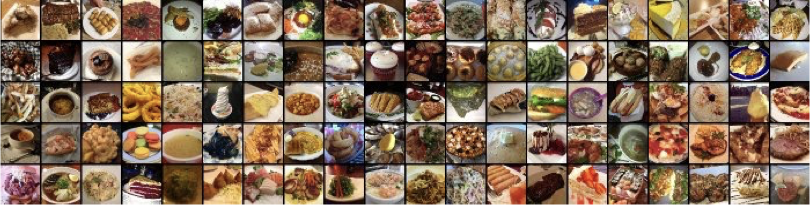
\includegraphics[width=1\linewidth]{images/food101dataset-image.png}
\end{center}

The Food-101 dataset, created by the Visual Computing Group at ETH Zurich, is a benchmark collection of images for machine learning models in food recognition tasks. This dataset comprises 101,000 images, evenly distributed across 101 different food categories where each category contains 1000 images. These are real-life images, varying in angles, presentation, lighting conditions, and backgrounds, all of which add complexity to the dataset. All images are rescaled to have a maximum side length of 512 pixels. We have further resized the image to 256x256 and taken a 224x224 center crop to reduce the computation time for all the models.

\subsubsection{Category Distribution}
Each of the 101 categories in the Food-101 dataset is represented by 1000 images, ensuring a uniform distribution across categories. Examples of these categories include foods like pizza, sushi, and apple pie, showcasing the dataset's diversity.

\subsubsection{Training/Test Split}
The dataset is pre-divided into training and test sets, with 750 training images and 250 test images per class. This results in a total of 75,000 images in the training set and 25,000 images in the test set. Instead of using the predetermined split, we split the dataset with a 70/20/10 split for training, validation and testing.

\subsubsection{Example Images from the Dataset}

\begin{center}
    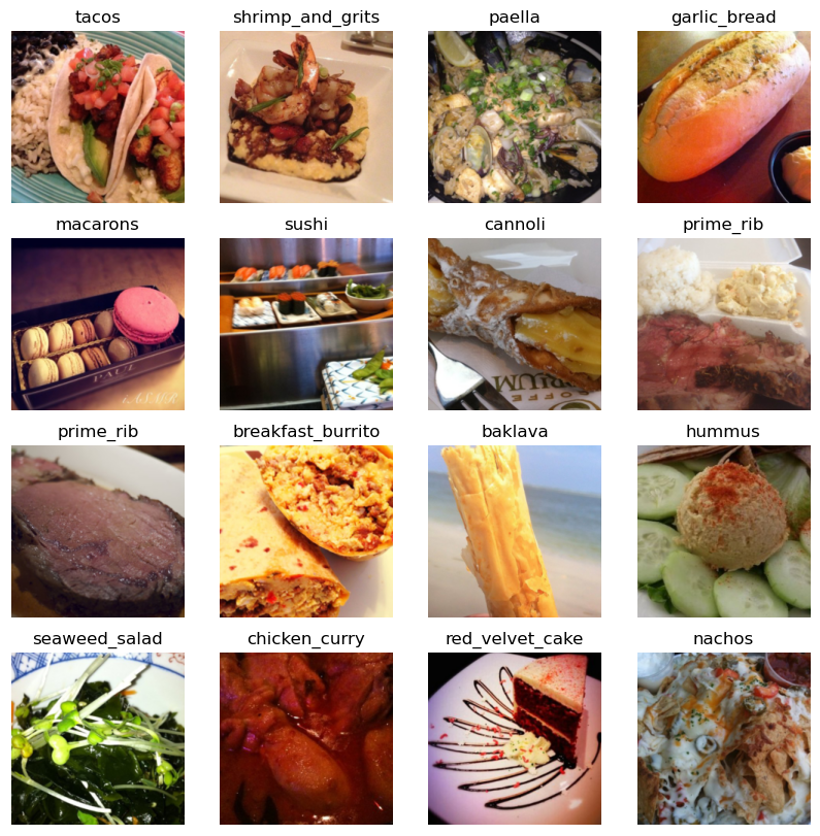
\includegraphics[width=0.7\linewidth]{images/example-dataset-images.png}
\end{center}

\subsection{Models chosen for training}

We used the following models for training:
\begin{itemize}
    \item EfficientNetV2
    \item ResNet50
    \item VGG16
    \item MobileNetV3
    \item DenseNet121
\end{itemize}

Each model is both fine-tuned and trained from scratch for 10 epochs. We chose these models in order to have a variety of CNNs varying in complexity, architecture and size to see how that affects learning in this food classification context. We also wanted to see how far we can get without pre-training to help the learning process.

\subsection{Data Loading and Preprocessing}

We initiated the process with the integration of essential Python libraries aimed at data handling and model development. The main part of the project i.e., neural network is imported from pytorch as "nn" and to fine-tune our models, we have included optimization utilities from \verb|torch.optim|.

To augment computational efficiency, we have used \verb|torch.cuda.amp| for Automatic Mixed Precision which gives us a good balance between speed and model performance. We use PyTorch's \verb|Resize| and \verb|CenterCrop| functions for data preprocessing. \verb|sklearn.metrics| is used to assess model accuracy and performance. 

Data exploration and visualization are conducted using Pandas and Matplotlib. Our progress through lengthy iterations is visually tracked via \verb|tqdm|'s progress bars, enhancing our experimental monitoring.

The \verb|datetime| module assists us in logging and time-stamping which was important for maintaining a chronological record of the experimentation. We use the timestamp for saving the pickle files containing the model metrics and the testing results.

We have kept the data split of 70-20-10 for train, validation and test loaders. Also, we have kept the batch size of 256 and have used 8 workers to decrease the processing time.

\subsection{Implementation Details}
We have established a training procedure  train\_and\_validate\_model , to accommodate a model, data loaders for training and validation, and the number of epochs for the iterative training process. Our model's environment is set to utilize CUDA capabilities, thereby leveraging GPU acceleration when available, with a fallback to CPU otherwise.

The training leverages the Adam optimizer with a learning rate set at 0.001. We further refine the learning process with a learning rate scheduler implementing a step decay policy, reducing the learning rate by a factor of 0.1 every 7 epochs to fine-tune the convergence. Since we are running for 10 epochs, the learning rate will be reduced once.

Our model employs the CrossEntropyLoss function, suitable for classification tasks with multiple classes. During training, gradient scaling is used to combat the vanishing gradient problem which is beneficial when training with mixed precision.

We set the number of training epochs to 10, with per-epoch metrics for losses and accuracies being tracked to monitor the model's performance over time. Each epoch iterates over the training data, making use of the tqdm library to provide a progress bar that shows us the training duration and progress.

In our project, the models we have used are EfficientNetV2, ResNet50, VGG16, MobileNetV3, and DenseNet121.  The \verb|get_model| function retrieves these models with pre-trained weights for transfer learning or loads them without any weights based on the parameter passed in.  The \verb|modify_model_classes| function subsequently customizes each model's classifier to accommodate the specific number of classes in our dataset, which is 101. This approach ensures that each model is fine-tuned to our classification objectives, allowing for a comprehensive comparative analysis across different network architectures.

\subsection{Model architecture}

The model architecture utilized in our experiments makes use of various CNN structures. Each model features a distinctive network structure optimized for achieving high accuracy in visual recognition tasks.

\subsubsection*{EfficientNetV2}
EfficientNetV2 is architected with a compound scaling method that scales the dimensions of depth, width, and resolution uniformly. It uses mobile inverted bottleneck convolutions (MBConv), similar to MobileNetV3, optimized for scaling and efficiency, and includes Fused-MBConv blocks for enhanced training speed.

\subsubsection*{ResNet50}
ResNet50 is a member of the Residual Network family and employs skip connections to allow inputs to bypass some layers. The network is 50 layers deep, comprising convolutional layers, batch normalization, ReLU activations, and residual blocks, which mitigate the vanishing gradient problem in deep networks.

\subsubsection*{VGG16}
VGG16's architecture is characterized by its simplicity, using a sequence of convolutional layers with 3x3 filters, max pooling, and three fully connected layers at the end. The activation function used is ReLU, and the network's depth compensates for the small receptive fields of the convolutional filters.

\subsubsection*{MobileNetV3}
MobileNetV3, optimized for mobile devices, incorporates depthwise separable convolutions, squeeze-and-excitation blocks, and the h-swish activation function. Its architecture is the product of a neural architecture search (NAS), focusing on efficiency and performance.

\subsubsection*{DenseNet121}
DenseNet121 utilizes dense connectivity, connecting each layer to every other layer in a feed-forward fashion. The network consists of dense blocks and transition layers for downsampling, promoting feature reuse, and reducing the vanishing gradient issue.

For our specific tasks, these models were initialized with pre-trained weights and modified at their classifier heads to accommodate the number of classes in our dataset. The EfficientNet's and ResNet50's classifiers were replaced with a linear layer tailored to our class count, while VGG16's sixth classifier layer, MobileNetV3's third classifier layer, and DenseNet121's classifier were all adapted accordingly. This modification ensures the networks' output layers are attuned to produce probabilities across our dataset's 101 distinct classes, making the architectures well-suited for our classification tasks.

\section{Experiment results}

\subsection*{Pre-trained Models Accuracy and Loss}

\begin{center}
    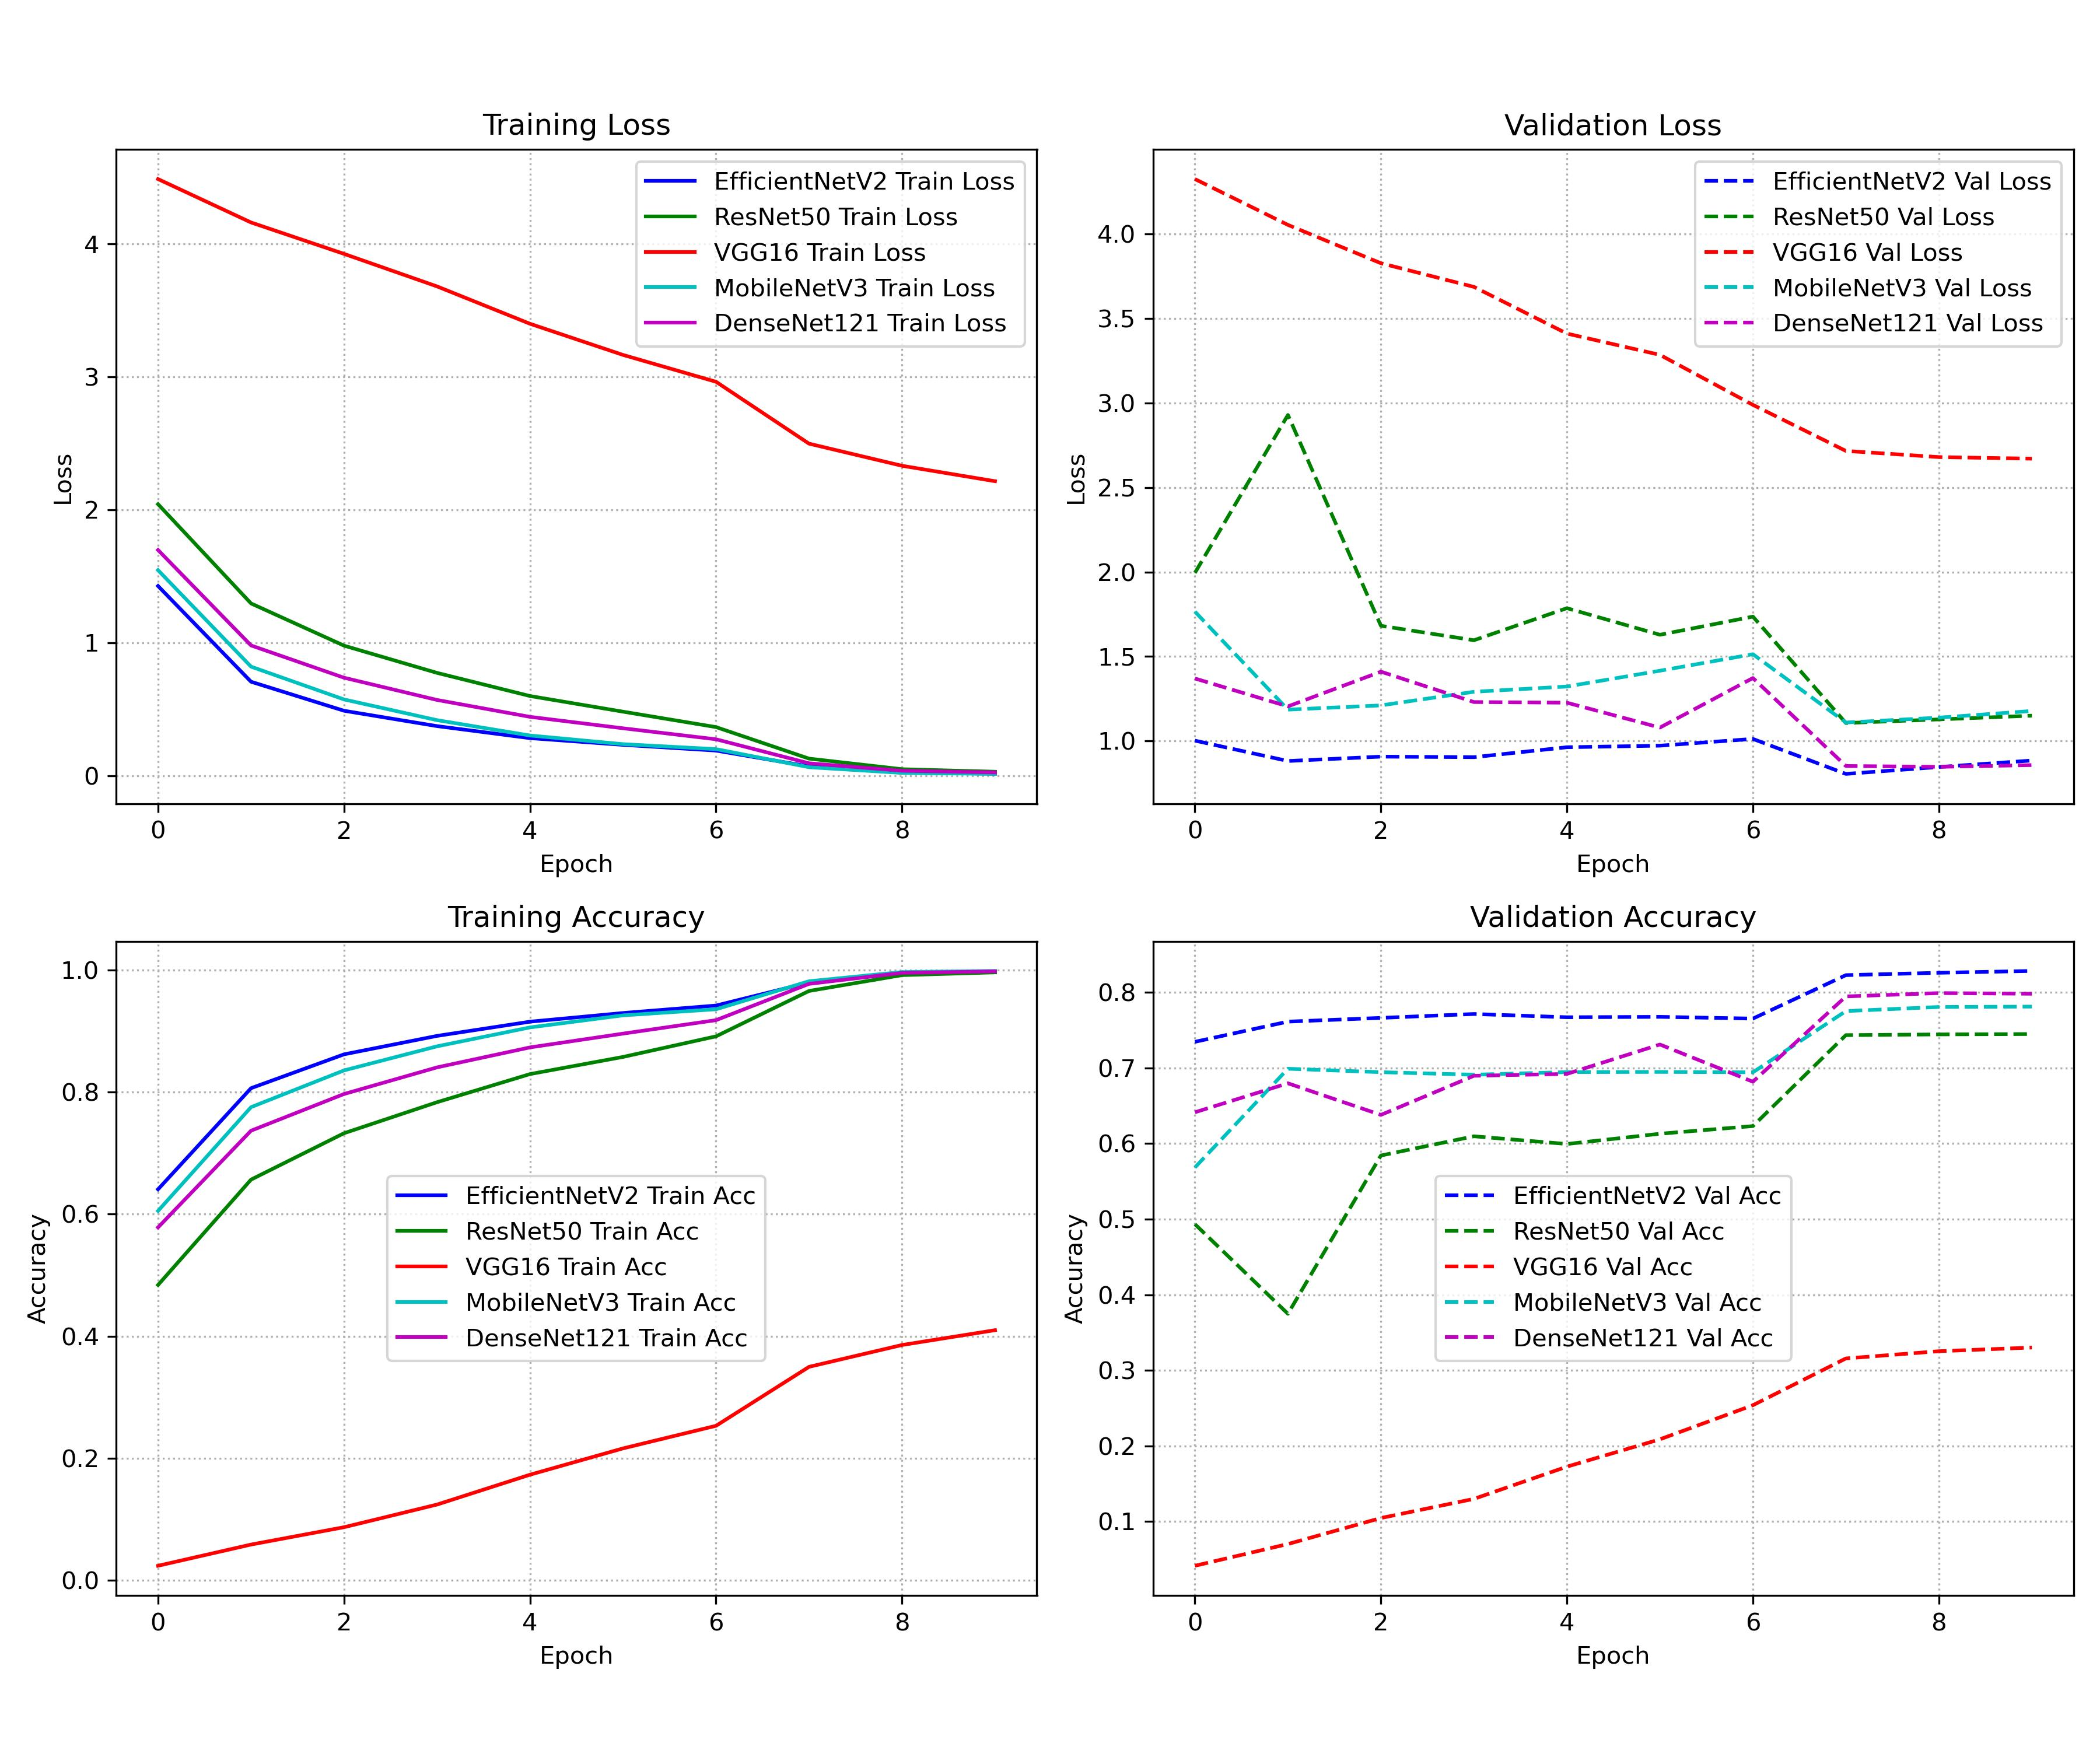
\includegraphics[width=1\linewidth]{images/pt_models.jpg}
\end{center}

Analyzing the pretrained models' performance on the Food-101 dataset, we see that EfficientNetV2 starts with a high training loss which rapidly decreases, indicating an effective adaptation to the dataset after the initial epochs. DenseNet121 exhibits a stable and consistent decline in training loss, suggesting a robust transfer of features with minimal overfitting. In contrast, VGG16, while improving, shows a higher loss throughout the training process, pointing to a less efficient transfer learning process on this specific dataset. After 6 epochs training loss for all the models except VGG16 tends to zero.

When examining validation losses, DenseNet121 and MobileNetV3 show a smoother curve with less volatility, which is indicative of a better generalization compared to VGG16, which exhibits higher peaks which suggest that it may not be as adept at generalizing the learned features to new data. This is further supported by the validation accuracy graph, where DenseNet121 and MobileNetV3 achieve higher accuracy, while VGG16 lags behind, indicating its relative ineffectiveness at classifying the Food-101 images despite the use of pretrained weights.

Overall, 4 of the 5 models we tested are reasonably close in performance. The outlier here is VGG16 which was clearly not able to handle the images in this dataset.



\subsection*{Non-Pretrained Models Accuracy and Loss}

\begin{center}
    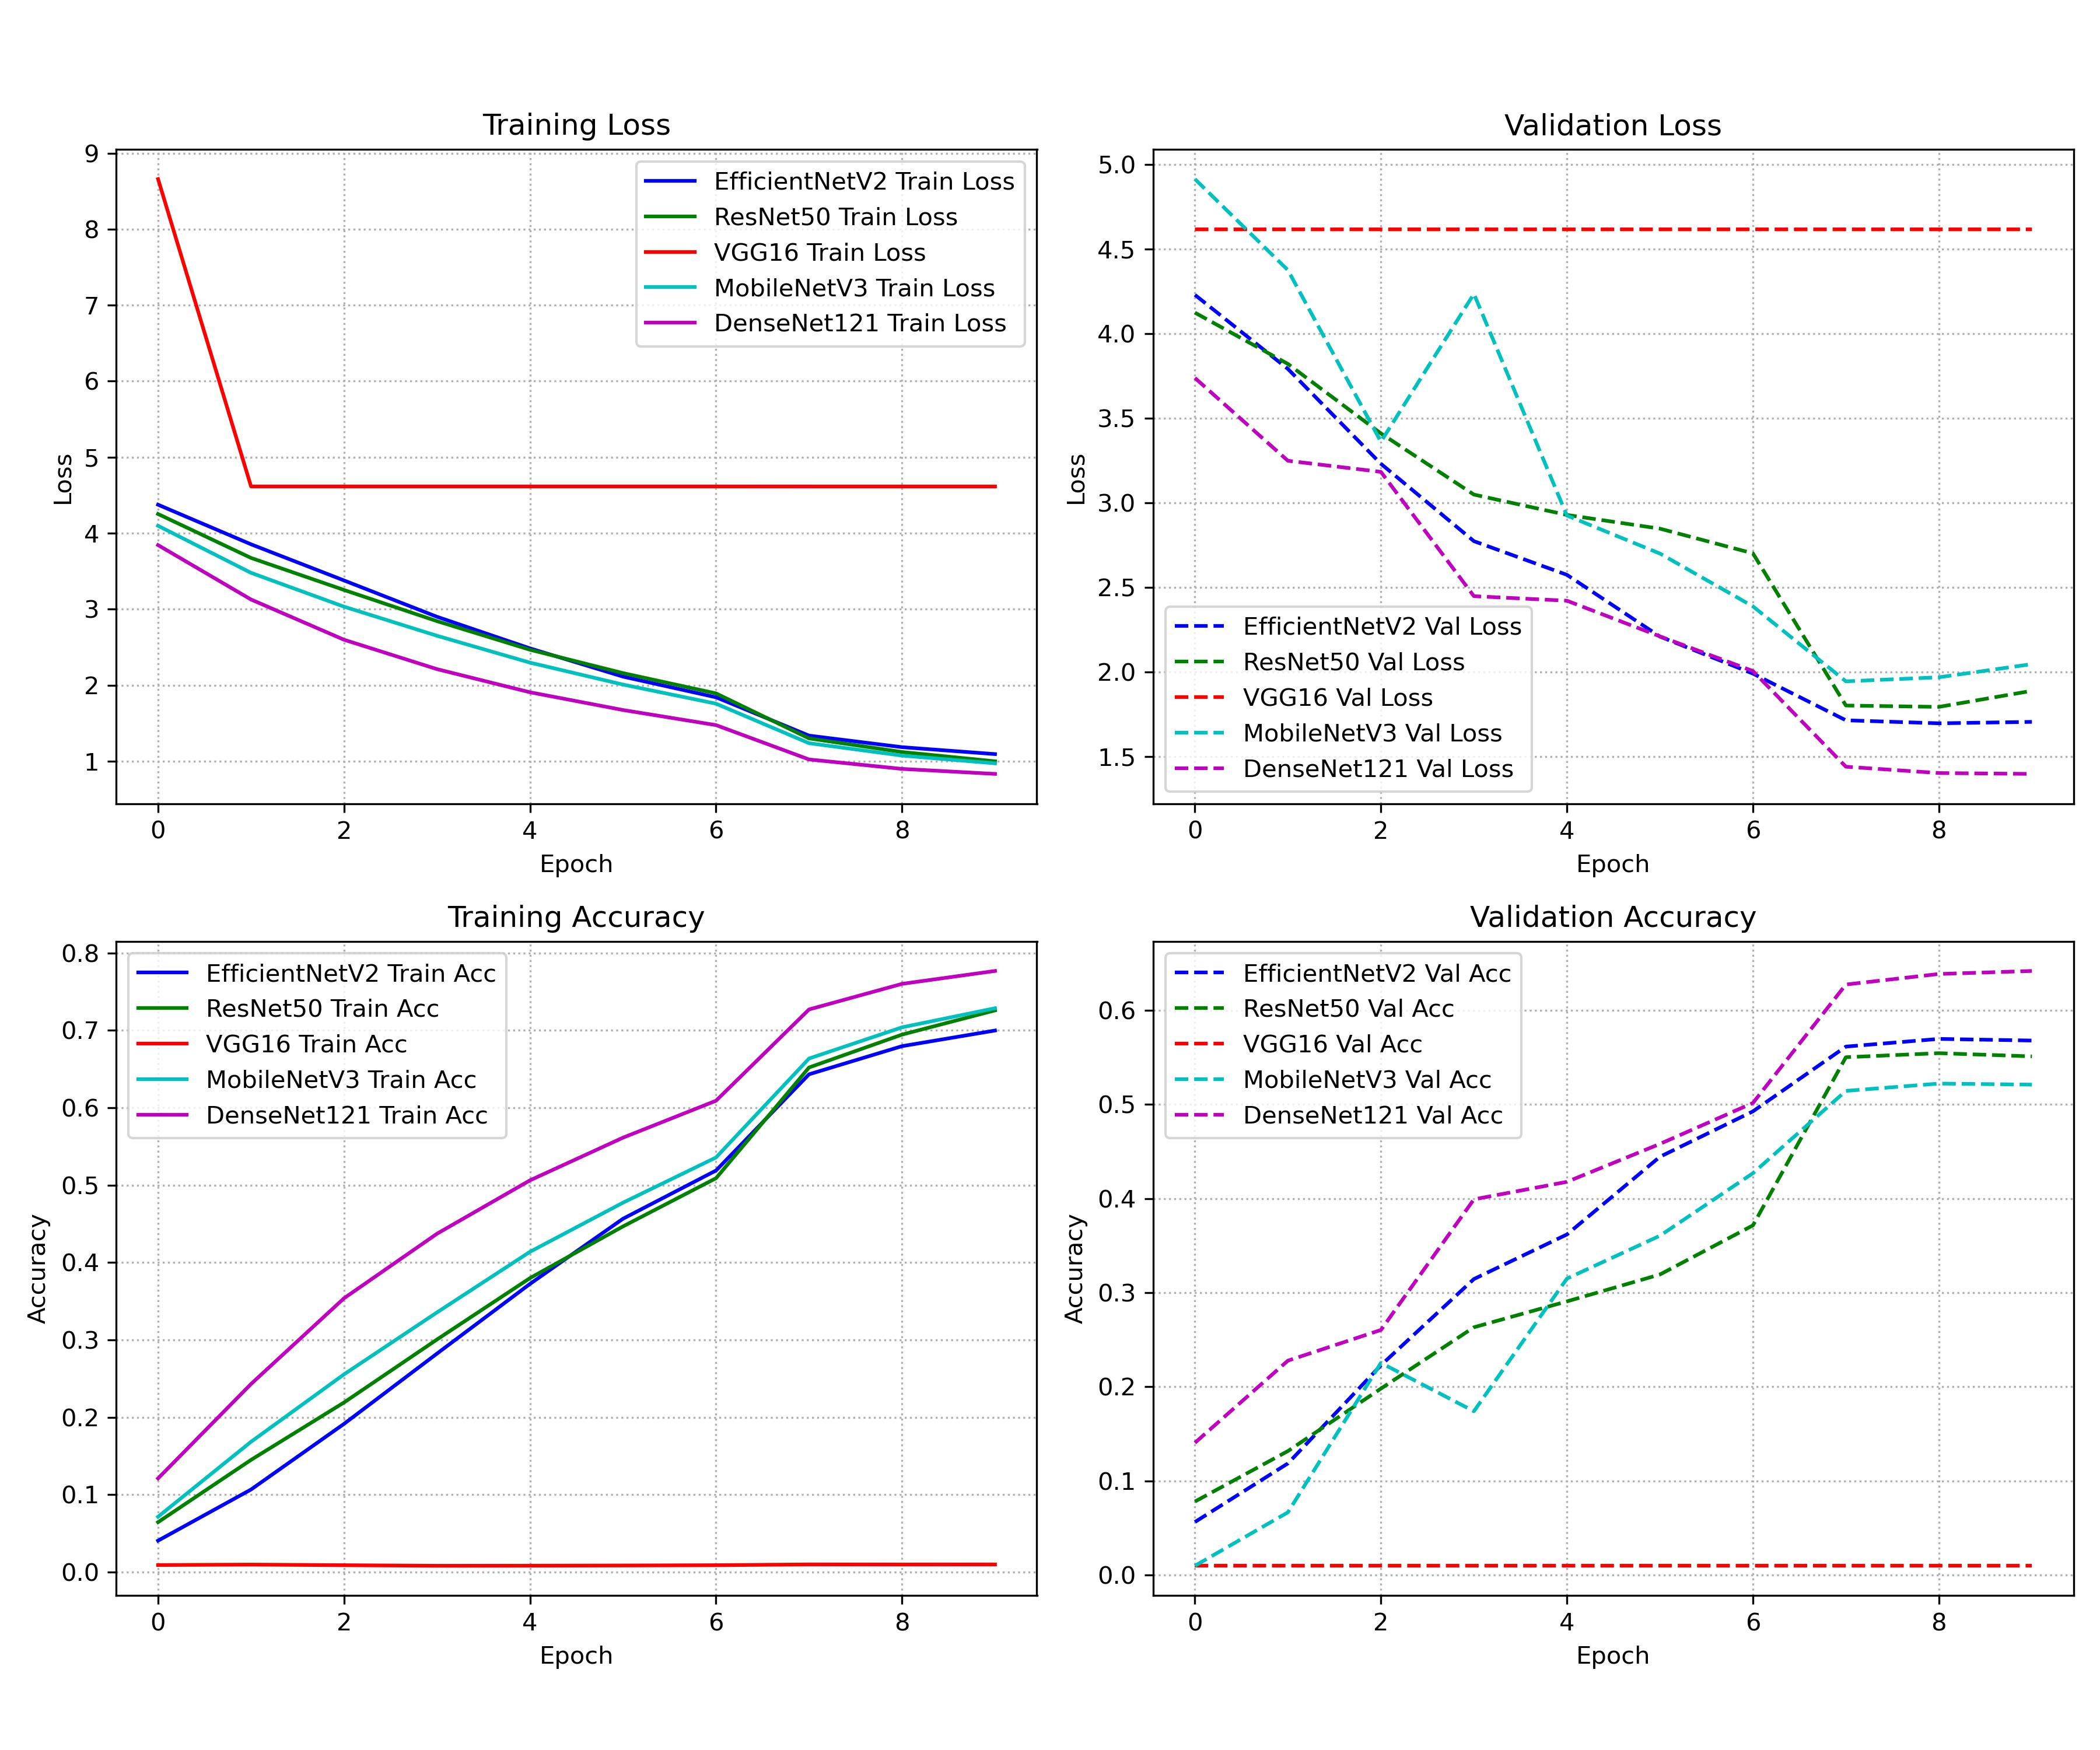
\includegraphics[width=1\linewidth]{images/npt_models.jpg}
\end{center}

For the non-pretrained models, the training loss graph shows that all models except VGG16 improve over time, with DenseNet121 and MobileNetV3 indicating a steady learning process. However, VGG16 stands out for its poor performance, with a training loss that plateaus early on and remains there throughout the rest of the epochs. This could be due to the model's architectural complexity and a higher number of parameters, which might not be as conducive to learning from scratch in a complex dataset like Food-101.

The validation loss graph for non-pretrained models mirrors this trend, where VGG16 shows a higher loss which is constant, that suggest the model is not learning anything. In terms of accuracy, VGG16's performance is notably poorer than that of DenseNet121 and MobileNetV3, which manage to achieve higher validation accuracies, reflecting a better aptitude for learning discriminative features without the aid of pretrained weights. This huge difference in the performance of VGG16, when compared to DenseNet121 and MobileNetV3, highlights the importance of choosing the right architecture when pretraining is not an option, as some models are inherently better at learning from scratch than others.

We are not entirely sure why the training loss and accuracy plateaus like this. We tried a few training runs with adjusted learning rates, and the accuracy was a little better (around 5\%) but we could not do many more runs to get a definite answer, as each execution of the code where all models get trained was taking a few hours.

For both pretrained and non-pretrained models, we used the Adam optimizer with an initial learning rate of 0.001. We experimented with only a couple other initial learning rates (0.01 and 0.0001) since each time we ran the code, it would take multiple hours for the 5 models to get trained both with and without pretraining and since we also had StepLR running at epoch 7. From these three, 0.001 worked best for most of the models (except VGG in the non-pretrained case).

Similar to the pretrained model results, 4 of the 5 models we tested are reasonably close in performance.

\subsection*{Results on Test Set}
\begin{table}[!ht]
    \centering
    \caption{Performance Metrics for Pretrained Models}
    \begin{tabular}{|l|l|l|l|l|l|l|}
        \hline
        \textbf{} & \textbf{Model} & \textbf{Pretrained} & \textbf{Precision} & \textbf{Recall} & \textbf{F1 Score} & \textbf{Accuracy} \\ \hline
        0 & EfficientNetV2 & True & \textbf{0.8293} & \textbf{0.8276} & \textbf{0.8275} & \textbf{0.8276} \\ \hline
        1 & ResNet50 & True & 0.7514 & 0.7480 & 0.7485 & 0.7480 \\ \hline
        2 & VGG16 & True & 0.3173 & 0.3301 & 0.3191 & 0.3301 \\ \hline
        3 & MobileNetV3 & True & 0.7793 & 0.7778 & 0.7780 & 0.7778 \\ \hline
        4 & DenseNet121 & True & 0.8000 & 0.7983 & 0.7982 & 0.7983 \\ \hline
    \end{tabular}
\end{table}

\begin{table}[!ht]
    \centering
    \caption{Performance Metrics for Non-Pretrained Models}
    \begin{tabular}{|l|l|l|l|l|l|l|}
    \hline
        \textbf{} & \textbf{Model} & \textbf{Pretrained} & \textbf{Precision} & \textbf{Recall} & \textbf{F1 Score} & \textbf{Accuracy} \\ \hline
        0 & EfficientNetV2 & False & 0.5748 & 0.5743 & 0.5716 & 0.5743 \\ \hline
        1 & ResNet50 & False & 0.5637 & 0.5524 & 0.5510 & 0.5524 \\ \hline
        2 & VGG16 & False & 0.0001 & 0.0099 & 0.0002 & 0.0099 \\ \hline
        3 & MobileNetV3 & False & 0.5215 & 0.5202 & 0.5171 & 0.5202 \\ \hline
        4 & DenseNet121 & False & \textbf{0.6458} & \textbf{0.6421} & \textbf{0.6412} & \textbf{0.6421} \\ \hline
    \end{tabular}
\end{table}

As we saw in the graph results, for pre-trained models, EfficientNetV2 performs the best while VGG16 performs worst and for non pre-trained models, DenseNet121 performs best while VGG16 performs the worst. Hence, we can say that, when we train these models from scratch, DenseNet121 performs best while among the pre-trained models EfficientNetV2 is best. In both cases, VGG16 performs the worst.

\subsubsection*{Results on Food-11 Test Set}

Prior to running these models on the larger Food-101 dataset, we first decided to try training them on a much smaller dataset called Food-11. This dataset contains 11 broad categories of food, namely Bread, Dairy product, Dessert, Egg, Fried food, Meat, Noodles-Pasta, Rice, Seafood, Soup and Vegetable-Fruit, and contains 16643 images in total (roughly 16.5\% the size of Food-101).

Results on Food-11 also show a similar pattern, with EfficientNetV2 performing the best among the pre-trained models and DenseNet121 performing the best among the non pre-trained ones. However we can see that across the board, the performance is higher on this dataset. Perhaps having fewer but broader categories makes it easier for the models to get their guesses right. Additionally, some food items in the same category could have common properties like texture, color, etc. which can help in making the correct prediction.

\begin{table}[!ht]
    \centering
    \caption{Food-11 Performance Metrics for Pretrained Models}
    \begin{tabular}{|l|l|l|l|l|l|l|}
    \hline
        ~ & Model & Pretrained & Precision & Recall & F1 Score & Accuracy \\ \hline
        0 & EfficientNet & True & \textbf{0.9407} & \textbf{0.9405} & \textbf{0.9404} & \textbf{0.9405} \\ \hline
        1 & ResNet & True & 0.8833 & 0.8838 & 0.8833 & 0.8838 \\ \hline
        2 & VGG & True & 0.5951 & 0.5946 & 0.5885 & 0.5946 \\ \hline
        3 & MobileNet & True & 0.9287 & 0.9283 & 0.9282 & 0.9283 \\ \hline
        4 & DenseNet & True & 0.9245 & 0.9241 & 0.9240 & 0.9241 \\ \hline
    \end{tabular}
\end{table}

\begin{table}[!ht]
    \centering
    \caption{Food-11 Performance Metrics for Non-pretrained Models}
    \begin{tabular}{|l|l|l|l|l|l|l|}
    \hline
        ~ & Model & Pretrained & Precision & Recall & F1 Score & Accuracy \\ \hline
        0 & EfficientNet & False & 0.6039 & 0.6074 & 0.6041 & 0.6074 \\ \hline
        1 & ResNet & False & 0.6380 & 0.6448 & 0.6401 & 0.6448 \\ \hline
        2 & VGG & False & 0.3868 & 0.3962 & 0.3836 & 0.3962 \\ \hline
        3 & MobileNet & False & 0.5982 & 0.5931 & 0.5930 & 0.5931 \\ \hline
        4 & DenseNet & False & \textbf{0.7376} & \textbf{0.7410} & \textbf{0.7382} & \textbf{0.7410} \\ \hline
    \end{tabular}
\end{table}

\section{Result Comparison with Existing Models}

Our project used EfficientNetV2, ResNet50, VGG16, MobileNetV3, and DenseNet121, achieving a top accuracy of 82.76\% with EfficientNetV2 when pretrained. This is good result considering the complexity of the Food-101 dataset and limited time and resources. When we compare this to the current SOTA models, Bamboo (ViTB/16) leads with 92.9\% accuracy, followed by SEER (RegNet10B - linear eval) at 90.3\%, and TWIST (ResNet-50) at 89.3\%. These models likely benefit from larger and more diverse training datasets, sophisticated architectures, and advanced training regimes.

Notably, our DenseNet121's performance, at 79.83\% accuracy, closely approaches that of TransBoost-ResNet50, which stands at 84.30\%. It is important to note that none of our models used extra training data, which is generally used by top-ranking models to boost performance. We are using the results found on the Food-101 benchmark on Papers with code (reference link below).

Our findings emphasize the potential use of these strategies in future endeavors to bridge the gap with state-of-the-art (SOTA) models. Additionally, we aim to delve into the innovative methodologies responsible for achieving these remarkable levels of accuracy. Techniques like data augmentation may help in further making the models more robust, and we could use Grad-CAM to see what features the CNN models are actually learning, and making changes to our training pipeline based on those findings.

\section{Food Generation using Diffusion Model Trained from Scratch}

In our project, we also tried out image generation, specifically focusing on creating images of food. We were curious to see how a diffusion model built from the scratch would perform in crafting pictures of various dishes.  To be particular, we generated pizza images using a UNet2DModel over 100 epochs. We originally wanted to generate different categories but were time and resource constrained.

\textbf{Model Configuration:} We defined \verb|TrainingConfig| with parameters like image size, batch sizes, epochs, learning rate, and more. The model generates 128x128 pixel resolution images.

\textbf{Data Preparation:} The dataset, specifically \verb|food101|, is filtered to focus on pizza images. A transformation pipeline is applied, including resizing, flipping, and normalization.

\textbf{Model Architecture:} The diffusion model used is a U-Net architecture, a type of CNN which is used in image generation tasks. It is set up with specific configurations like in/out channels, layers per block, and block types for both downsampling and upsampling.

\textbf{Training Process:} The training involves creating noisy versions of the images and then learning to denoise them. Loss is computed using mean squared error (MSE), and we use an AdamW optimizer with a cosine schedule for learning rate adjustment. Most of the hyperparameters are the same as the ones in the Huggingface documentation for training diffusion models from scratch. This was only a short experiment that we conducted towards the end of the project, so we did not get a lot of time to try out hyperparameter tuning since running the training for 100 epochs was taking a very long time in addition to the wait time for high VRAM GPUs on the Discovery Cluster.

\textbf{Output of Pizza Images:}

\begin{center}
    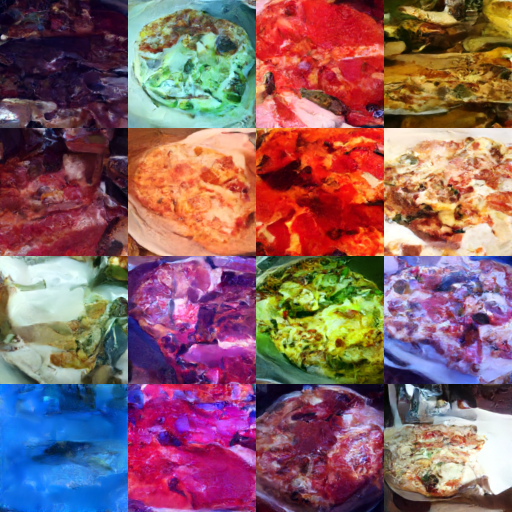
\includegraphics[width=0.7\linewidth, height=0.6\linewidth]{images/generated-pizza-images.png}
\end{center}

The image above shows 16 pizza images generated by our model, trained on the Pizza images in the Food-101 dataset. For the short amount of time we trained it, and the relatively small number of images we are quite happy with the result and more improvements can definitely be made to this model to generate more realistic images. Additionally, using a pretrained model like Stable Diffusion or other Diffusion models would most likely improve the performance here, but we specifically wanted to try training one from scratch to see how well it could do given limited resources.

\section{Conclusion}

In conclusion, our project on Food Image Classification and Generation demonstrated the potential and challenges of applying deep learning models to the complex task of food image recognition. We successfully trained models like EfficientNetV2, ResNet50, VGG16, MobileNetV3, and DenseNet121, achieving noteworthy results, especially with EfficientNetV2 in the pretrained category. The project highlighted the effectiveness of transfer learning and the importance of model selection. Despite not reaching state-of-the-art accuracies, our findings provide a strong foundation for future research, particularly in fine-tuning model parameters and exploring more sophisticated training strategies.  Additionally, our experiment with creating pizza pictures using a self-trained diffusion model was an exciting step and a great learning opportunity for us. It really opened our eyes to what AI can do and can't do when it comes to creative stuff like making images. In conclusion, this project highlights the changing landscape of AI in food-related applications, paving the way for ongoing exploration and innovation in the field.

\section{References}

\begin{enumerate}
    \item Food-101 Paper: \small{\url{https://data.vision.ee.ethz.ch/cvl/datasets_extra/food-101/static/bossard_eccv14_food-101.pdf}}
    \item Food-101 Dataset Website: \small{\url{https://data.vision.ee.ethz.ch/cvl/datasets_extra/food-101/}}
    \item Food-101 Dataset Kaggle Link: \small{\url{https://www.kaggle.com/datasets/dansbecker/food-101}}
    \item Food-11 Dataset Link: \small{\url{https://www.kaggle.com/datasets/trolukovich/food11-image-dataset}}
    \item Food-101 Benchmark: \small{\url{https://paperswithcode.com/sota/image-classification-on-food-101-1}}
    \item PyTorch Documentation: \small{\url{https://pytorch.org/tutorials/beginner/blitz/cifar10_tutorial.html}}
    \item Huggingface Diffusers Documentation: \small{\url{https://huggingface.co/docs/diffusers/tutorials/basic_training}}
    \item Huggingface Diffusers Code: \small{\url{https://github.com/huggingface/diffusers/tree/v0.24.0/src/diffusers}}
\end{enumerate}

\end{document}
